%! suppress = FileNotFound
\documentclass[titlepage]{article}

\usepackage[utf8]{inputenc}
\usepackage[letterpaper, portrait, margin=1in]{geometry}
\usepackage{graphicx} % Required for inserting images
\usepackage{amsmath}
\usepackage{float}
\usepackage{indentfirst}
\usepackage{hyperref}
\usepackage{settobox}

\graphicspath{{./latex\_figures/}}

\title{Spring Potential Energy Lab}
\author{Aiden Ma}
\date{October 17th, 2023}

\begin{document}
    
    \maketitle
    
    \tableofcontents
    
    \newpage
    
    
    \section{Introduction}\label{sec:introduction}
        In this lab, we will be investigating the rate of change of mechanical energy over time of an oscillating mass on a spring.
        We will measure the spring constant of the spring, as well as the position and velocity of the mass oscillating vertically on a spring.
    
    
    \section{Relevant Knowledge}\label{sec:relevant-knowledge}
        \begin{itemize}
            \item \textbf{Mechanical energy} is the sum of kinetic energy and potential energy.
            Mechanical energy is measured in joules (J).
            \item \textbf{Kinetic energy} is the energy of motion.
            The equation for kinetic energy is $K = \frac{1}{2}mv^2$, where $m$ is the mass of the object and $v$ is the velocity of the object.
            Kinetic energy is measured in joules (J).
            \item On the other hand, \textbf{potential energy} is the energy an object possesses due to its position relative to others.
            Potential energy is stored energy that can be converted into kinetic energy.
            There are many forms of potential energy, two of which are relevant to this lab.
            \begin{itemize}
                \item \textbf{Spring potential energy} is the energy stored in a spring when it is stretched or compressed from its equilibrium position.
                The equation for spring potential energy is $U = \frac{1}{2}k(\Delta x)^2$, where $k$ is the spring constant and $\Delta x$ is the distance the spring is stretched.
                \item \textbf{Gravitational potential energy} is the energy stored in an object due to its position another position.
                The equation for gravitational potential energy is $U = mgh$, where $m$ is the mass of the object, $g$ is the acceleration due to gravity, and $h$ is the height of the object relative to another position ($h = x-x_0$).
            \end{itemize}
            \item The \textbf{spring constant} is the force required to stretch the spring 1 meter.
            The unit for spring constant is newtons per meter ($\frac{\text{N}}{\text{m}}$).
            \item A \textbf{cycle} is one complete oscillation of the spring from peak to peak.
            \item A \textbf{peak} is the highest point of the oscillation.
        \end{itemize}
    
    
    \section{Goal}\label{sec:goal}
        To determine the rate of change of mechanical energy with respect to time of a mass oscillating vertically by the use of a spring.
    
    
    \section{Materials}\label{sec:materials}
        \begin{itemize}
            \item Laptop with Logger Pro
            \item Spring
            \item 3x 20g masses
            \item 1x 50g mass
            \item Ultrasonic motion detector
            \item Ruler
            \item Mass holder
            \item Stand
            \item Test tube clamp
        \end{itemize}
    
    
    \section{Procedure}\label{sec:procedure}
        \noindent Part 1: Measuring the spring constant:
        \begin{enumerate}
            \item Set up the spring so that it is hanging vertically from the stand, with the ruler measuring the bottom of the spring at position 0.
            There should be no mass attached to the spring except for the mass holder.
            \item Add the 20g mass to the spring and record the length of the spring.
            \item Repeat step 3 until all 3 20g masses are added.
            \item Remove all the masses and add the 50g mass to the spring and record the length of the spring.
            \item Add a 20g mass to the spring and record the length of the spring.
        \end{enumerate}
        
        \noindent Part 2: Measuring the rate of change in mechanical energy over time:
        \begin{enumerate}
            \item Set up the stand so that the spring is hanging vertically directly above the ultrasonic motion detector.
            \item Open logger pro and set up the motion detector.
            \item Set up the spring so that it is at its equilibrium position.
            \item Record the position of the spring.
            \item Add a 50g mass to the spring, let the mass rest in its equilibrium position while not oscillating, and record the position of the spring.
            \item Pull the mass down 5cm and release it.
            \item Activate LoggerPro and record the position of the spring every 0.05 seconds using the ultrasonic motion detector for 415 seconds.
        \end{enumerate}
    
    
    \section{Data}
        
        \subsection{Spring extension with different masses}\label{subsec:spring-constant-data}
            The following table contains the length that the spring extended when different masses were added to it.
            The spring was measured where the zero was when the spring was at rest with only the mass holder (with mass $m_0$) attached.
            \begin{table}[H]
                \centering
                \small
                \begin{tabular}{|c|c|}
                    \hline
                    Mass ($m$) [kg]                & Length ($x$) [cm] \\
                    \hline
                    $m_0$                          & 0.00              \\
                    \hline
                    $m_0 + 0.02$ (1x 20g)          & 1.95              \\
                    \hline
                    $m_0 + 0.04$ (2x 20g)          & 3.90              \\
                    \hline
                    $m_0 + 0.05$ (1x 50g)          & 4.90              \\
                    \hline
                    $m_0 + 0.06$ (3x 20g)          & 5.85              \\
                    \hline
                    $m_0 + 0.07$ (1x 20g + 1x 50g) & 6.85              \\
                    \hline
                \end{tabular}
                \caption{Spring extention data}\label{tab:spring-extention-data}
            \end{table}
        
        \subsection{Length of $x_0$ and $x$}\label{subsec:length-of-x0 and x}
            Experimentally the distance of $x_0$, the equilibrium point of the spring, above the motion detector was 32.8 cm.
            Experimentally, $x$, the rest length, is 24.0 cm above the motion detector.
        
        \subsection{Change in position and velocity of the oscillating mass over time}\label{subsec:change-in-position-and-velocity-of-the-oscillating-mass-over-time}
            %todo add a table of data
            
            The following are the graphs of the position and velocity of the oscillating mass over time:
            
            \begin{minipage}{.5\textwidth}
                \begin{figure}[H]
                    \centering
                    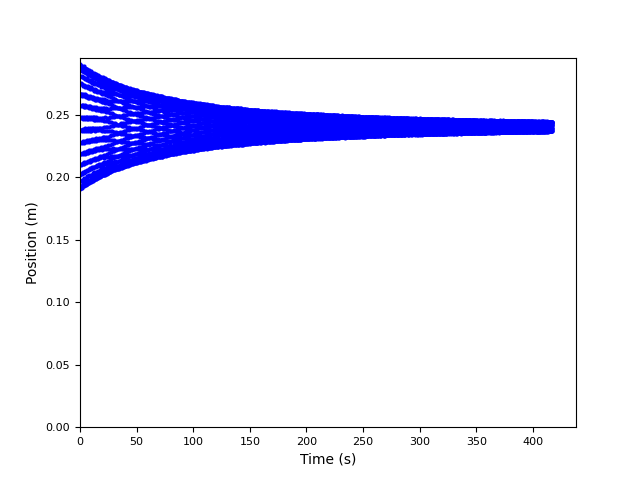
\includegraphics[width=\linewidth]{position}
                    \caption{Position of the oscillating mass over time}
                    \label{fig:position}
                \end{figure}
            \end{minipage}%
            \begin{minipage}{.5\textwidth}
                \begin{figure}[H]
                    \centering
                    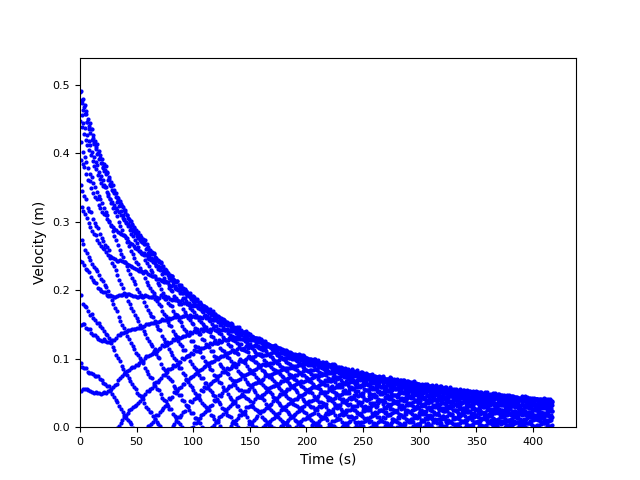
\includegraphics[width=\linewidth]{velocity}
                    \caption{Velocity of the oscillating mass over time}
                    \label{fig:velocity}
                \end{figure}
            \end{minipage}
    
    
    \section{Analysis}\label{sec:analysis}
        
        \subsection{Calculating the spring constant}\label{subsec:calculating-the-spring-constant}
            %TODO add a graph showing linear fit of the spring constant data
            
            In the following calculations, the system is the mass holder, the added masses, the spring, and the earth.
            
            The following figure is a free body diagram of the system:
            %figure FBD
            \begin{figure}[H]
                \centering
                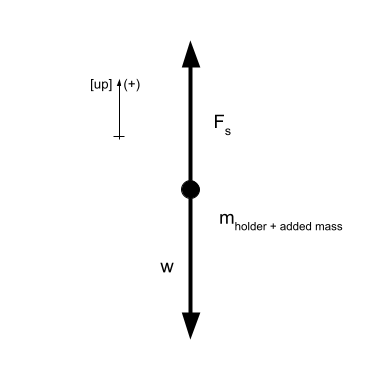
\includegraphics[width=0.3\linewidth]{FBD}
                \caption{Free body diagram of the mass holder and the added mass}
                \label{fig:FBD}
            \end{figure}
            
            Since the oscillating mass is at rest before and after adding the masses, $F_{net}^{\text{}} = 0$ and $F_{net}^{\text{'}} = 0$.
            Furthermore, the only force acting on the mass is gravity and the spring force and the mass is at rest, thus the spring force must be equal to the force of gravity.
            Therefore, we can calculate the spring constant:
            
            \begin{equation}
                \begin{aligned}
                    \small
                    F_{\text{net}}^{\text{'}} &= 0 \\
                    F_{\text{spring}}^{\text{'}} - F_{\text{gravity}}^{\text{'}} &= 0 \\
                \end{aligned}\label{eq:spring constant equation_pt1}
            \end{equation}
            
            Since $F_{net}^{\text{}} = 0$:
            \begin{equation}
                \begin{aligned}
                    \notag
                    \small
                    F_{\text{net}}^{\text{}} &= 0 \\
                    F_{\text{spring}}^{\text{}} - F_{\text{gravity}}^{\text{}} &= 0 \\
                \end{aligned}\label{eq:spring constant equation_pt2}
            \end{equation}
            
            Plugging back into equation~\ref{eq:spring constant equation_pt1} and solving for $k$:
            
            \begin{equation}
                \begin{aligned}
                    \small
                    F_{\text{spring}}^{\text{'}} - F_{\text{gravity}}^{\text{'}} &= 0 \\
                    F_{\text{spring}}^{\text{'}} - F_{\text{gravity}}^{\text{'}} &= F_{\text{spring}}^{\text{}} - F_{\text{gravity}}^{\text{}} \\
                    F_{\text{spring}}^{\text{'}} + F_{\text{gravity}}^{\text{}}- F_{\text{gravity}}^{\text{'}} - F_{\text{spring}}^{\text{}} &= 0 \\
                    \Delta F_{\text{spring}} - \Delta F_{\text{gravity}} &= 0 \\
                    \Delta F_{\text{spring}} &= \Delta F_{\text{gravity}} \\
                    k\Delta x &= g \Delta m \\
                    k &= \frac{g \Delta m}{\Delta x} \\
                \end{aligned}\label{eq:spring constant equation}
            \end{equation}
            
            %todo move tag to the end of the equation list
            
            In this case, $\Delta m$ is the mass of the mass added to the spring, and $\Delta x$ is the change in length of the spring when that mass is added.
            
            Using equation~\ref{eq:spring constant equation}, we can calculate the spring constant for each mass added to the spring.
            For example, if we take the data from the first mass, we can calculate the spring constant as follows:
            
            \begin{equation}
                \begin{aligned}
                    \small
                    \notag
                    k &= \frac{g \Delta m}{\Delta x} \\
                    k &= \frac{(9.8 \frac{\text{ m}}{\text{ s}^2})(0.02 \text{ kg})}{0.0195 \text{ m}} \\
                    k &= 10.05 \frac{\text{ N}}{\text{ m}} \\
                \end{aligned}\label{eq:example spring constant equation}
            \end{equation}
            
            The following table contains all the spring constants that were measured and is calculated using equation~\ref{eq:spring constant equation}:
            
            \begin{table}[H]
                \centering
                \small
                \begin{tabular}{|c|c|c|}
                    \hline
                    Added Mass ($m$) [kg] & Length ($\Delta x$) [m] & Spring Constant ($k$) [$\frac{\text{N}}{\text{m}}$] \\
                    \hline
                    0.02                  & 0.0195                  & 10.05                                               \\
                    \hline
                    0.04                  & 0.0390                  & 10.05                                               \\
                    \hline
                    0.05                  & 0.0490                  & 10.00                                               \\
                    \hline
                    0.06                  & 0.0585                  & 10.05                                               \\
                    \hline
                    0.07                  & 0.0685                  & 10.01                                               \\
                    \hline
                \end{tabular}
                \caption{Spring constant data}\label{tab:spring-constant-data}
            \end{table}
            
            Using this data, we can calculate the average spring constant:
            
            \begin{equation}
                \begin{aligned}
                    \small
                    k = k_{avg} &= \frac{k_1 + k_2 + k_3 + k_4 + k_5}{5} \\
                    k &= \frac{10.05 + 10.05 + 10.00 + 10.05 + 10.01}{5} \\
                    k &= 10.0 \frac{\text{ N}}{\text{ m}} \\
                \end{aligned}\label{eq:average spring constant equation}
            \end{equation} %TODO UPDATE THIS WITH MORE ACCURATE VALUES
            
            This matches with the linear regression of the spring constant data, which is $10.0 \frac{\text{ N}}{\text{ m}}$.
            %TODO add a graph showing linear fit of the spring constant data
        
        \subsection{Solving for the mass of the mass holder}\label{subsec:solving-for-the-mass-of-the-mass-holder}
            
            The mass of mass holder has a non-negligible impact on the overall mechanical energy of the system as the oscillating system includes the mass holder.
            The kinetic energy and the gravitational energy are both relative to the mass of the oscillating system, but the mass of the mass holder does not impact spring potential energy.
            This means that through a cycle, in order to calculate the correct mechanical energy, it is necessary to account for the mass of the mass holder. \\
            
            Using equation~\ref{eq:spring constant equation}, we can solve for the mass of the mass holder where $x_0$ is the equilibrium point of the spring.
            Using the values from in section~\ref{subsec:spring-constant-data} and section~\ref{subsec:calculating-the-spring-constant} as well as the value for $k$ from equation~\ref{eq:average spring constant equation} yields:
            
            \begin{equation}
                \begin{aligned}
                    \small
                    \notag
                    k &= \frac{g \Delta m}{\Delta x} \\
                    k &= \frac{g (m_{\text{mass holder}} + m_{\text{added mass}})}{x_0-x} \\
                    k(x_0-x) &= g (m_{\text{mass holder}} + m_{\text{added mass}}) \\
                    g(m_{\text{mass holder}} + m_{\text{added mass}}) &= k(x_0-x) \\
                    m_{\text{mass holder}} + m_{\text{added mass}} &= \frac{k(x_0-x)}{g} \\
                    m_{\text{mass holder}} &= \frac{k(x_0-x)}{g} - m_{\text{added mass}} \\
                    m_{\text{mass holder}} &= \frac{(10 \frac{\text{ N}}{\text{ m}})(0.328 \text{m} - 0.240 \text{ m})}{9.8 \frac{\text{ m}}{\text{ s}^2}} - 0.05 \text{ kg} \\
                    m_{\text{mass holder}} &= 0.04 \text{ kg} \\
                \end{aligned}\label{eq:mass-of-mass-holder-with-values}
            \end{equation}
            
            Therefore, the mass holder has a weight of 40 grams.
        
        \subsection{Calculating the mechanical energy}\label{subsec:calculating-the-mechanical-energy}
            The mechanical energy of the system is the sum of the kinetic energy and the potential energies.
            
            \subsubsection{Calculating gravitational potential energy}
                Gravitational potential energy is the energy stored in an object due to its position relative to another position.
                The equation for gravitational potential energy is $U = mgh$, where $m$ is the mass of the object, $g$ is the acceleration due to gravity, and $h$ is the height of the object relative to another position.
                
                If we let $h$ be the height of the mass relative to the equilibrium position when nothing is attached, then we can calculate the gravitational potential energy as follows:
                
                \begin{equation}
                    \begin{aligned}
                        \small
                        U_{\text{g}} &= mgh \\
                        U_{\text{g}} &= mg(x - 0.328 \text{ m}) \\
                        U_{\text{g}} &= (0.09 kg)(9.8 \frac{\text{ m}}{\text{ s}^2})(x - 0.328 \text{ m}) \\
                    \end{aligned}\label{eq:gravitational-potential-energy-equation}
                \end{equation}
                
                Using the data from section~\ref{subsec:change-in-position-and-velocity-of-the-oscillating-mass-over-time} and equation~\ref{eq:gravitational-potential-energy-equation}, we can calculate the gravitational potential energy for each data point.
                Figure~\ref{fig:gravitational-potential-energy} is a plot of the gravitational potential energy over time:
                
                %file in gravitational potential energy
                \begin{minipage}{.5\textwidth}
                    \begin{figure}[H]
                        \centering
                        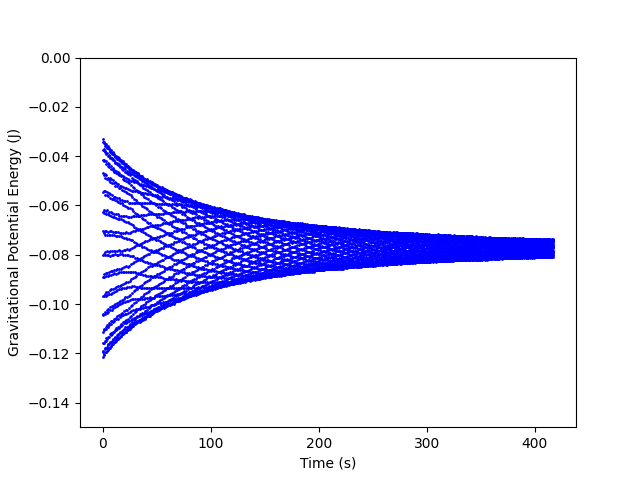
\includegraphics[width=\linewidth]{gravitational-potential-energy}
                        \caption{Gravitational potential energy over time}
                        \label{fig:gravitational-potential-energy}
                    \end{figure}
                \end{minipage}%
                \begin{minipage}{.5\textwidth}
                        %figure gravitational-potential-energy-zoomed
                    \begin{figure}[H]
                        \centering
                        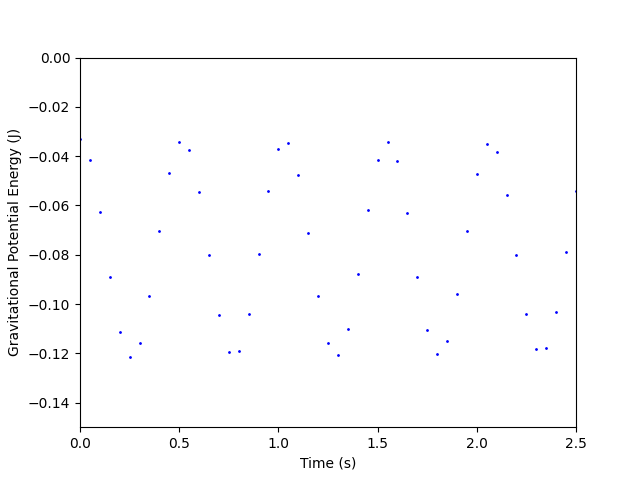
\includegraphics[width=\linewidth]{gravitational-potential-energy-zoomed}
                        \caption{Gravitational PE from 0 to 2.5 seconds}
                        \label{fig:gravitational-potential-energy-zoomed}
                    \end{figure}
                \end{minipage}\\
                
                
                One interesting thing to note is that in the gravitational potential energy graph (figure~\ref{fig:gravitational-potential-energy}) it looks like there are a series of lines at different heights.
                However, this is only a coincidence caused by the period of oscillation being extremely close to a multiple of the measuring interval of the motion detector.
                When the motion detector measures the position of the mass, the mass is at a similar position to when the motion detector measured exactly one cycle ago, thus the gravitational potential energy looks very similar to a previous point, but because they aren't the exact same, the slowly fall out of sync, explaining why the lines start to curve.
                Since this happens for multiple points in every cycle, the gravitational potential energy graph looks like a series of lines at different heights.
                
                Zooming in on a specific section, such as from 0 to 2.5 seconds in figure~\ref{fig:gravitational-potential-energy-zoomed}, shows how it is actually just a single line oscillating up and down.
            
            \subsubsection{Calculating spring/elastic potential energy}
                Spring potential energy is the energy stored in a spring when it is stretched or compressed.
                The equation for spring potential energy is $U = \frac{1}{2}k(\Delta x)^2$, where $k$ is the spring constant and $\Delta x$ is the distance the spring is stretched.
                
                \begin{equation}
                    \begin{aligned}
                        \small
                        U_{\text{s}} &= \frac{1}{2}k(\Delta x)^2 \\
                        U_{\text{s}} &= \frac{1}{2}(10 \frac{\text{ N}}{\text{ m}})(x_0 \text{ m} - x)^2 \\
                        U_{\text{s}} &= \frac{1}{2}(10 \frac{\text{ N}}{\text{ m}})(0.328 \text{ m} - x)^2 \\
                    \end{aligned}\label{eq:spring-potential-energy-equation}
                \end{equation}
                
                Using the data from section~\ref{subsec:change-in-position-and-velocity-of-the-oscillating-mass-over-time} and equation~\ref{eq:spring-potential-energy-equation}, we can calculate the spring potential energy for each data point.
                
                \begin{minipage}{.5\textwidth}
                        %figure elastic-potential-energy
                    \begin{figure}[H]
                        \centering
                        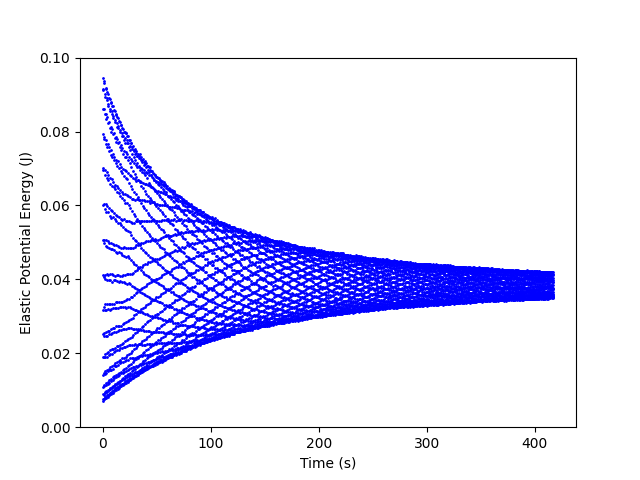
\includegraphics[width=\linewidth]{elastic-potential-energy}
                        \caption{Elastic potential energy over time}
                        \label{fig:elastic-potential-energy}
                    \end{figure}
                \end{minipage}%
                \begin{minipage}{.5\textwidth}
                        %figure elastic-potential-energy-zoomed
                    \begin{figure}[H]
                        \centering
                        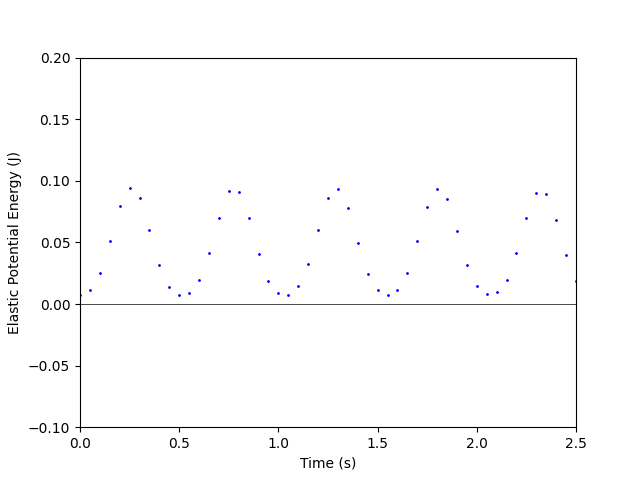
\includegraphics[width=\linewidth]{elastic-potential-energy-zoomed}
                        \caption{Elastic potential energy from 0 to 2.5 seconds}
                        \label{fig:elastic-potential-energy-zoomed}
                    \end{figure}
                \end{minipage}\\
                
                Just like in gravitational potential energy, the elastic potential energy graph looks like a series of lines.
                This is once again a coincidence caused by the period of the oscillating mass being extremely close to a multiple of the measuring interval.
                Zooming in on a specific section, such as from 0 to 2.5 seconds, clearly shows how it is just a single line oscillating up and down.
            
            \subsubsection{Calculating kinetic energy}
                
                The kinetic energy of an object is the energy that an object possesses due to its motion.
                The equation for kinetic energy is $K = \frac{1}{2}mv^2$, where $m$ is the mass of the object and $v$ is the velocity of the object.
                
                \begin{equation}
                    \begin{aligned}
                        \small
                        K &= \frac{1}{2}mv^2 \\
                        K &= \frac{1}{2}(0.09 \text{ kg})(v)^2 \\
                    \end{aligned}\label{eq:kinetic-energy-equation}
                \end{equation}
                
                Using the data from section~\ref{subsec:change-in-position-and-velocity-of-the-oscillating-mass-over-time} and equation~\ref{eq:kinetic-energy-equation}, we can calculate the kinetic energy for each data point.
                
                \begin{minipage}{0.5\textwidth}
                        %figure kinetic-energy
                    \begin{figure}[H]
                        \centering
                        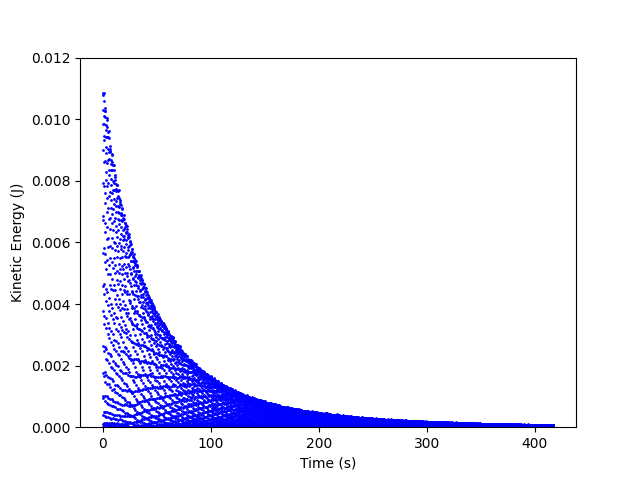
\includegraphics[width=\linewidth]{kinetic-energy}
                        \caption{Kinetic energy over time}
                        \label{fig:kinetic-energy}
                    \end{figure}
                \end{minipage}%
                \begin{minipage}{0.5\textwidth}
                        %figure kinetic-energy-zoomed
                    \begin{figure}[H]
                        \centering
                        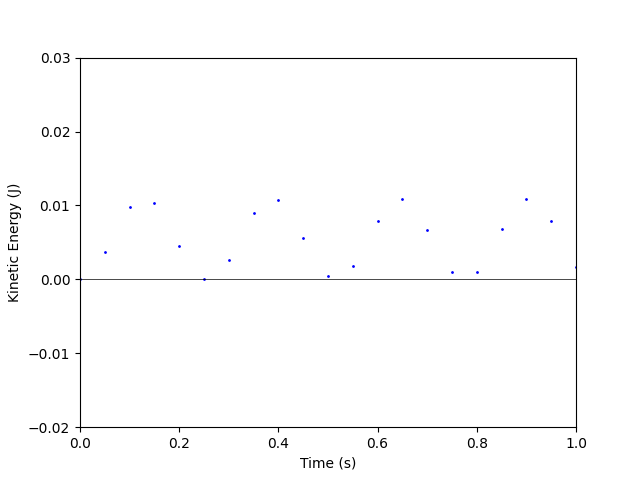
\includegraphics[width=\linewidth]{kinetic-energy-zoomed}
                        \caption{Kinetic energy from 0 to 1 second}
                        \label{fig:kinetic-energy-zoomed}
                    \end{figure}
                \end{minipage}\\
                
                Just like in gravitational potential energy and elastic potential energy, the kinetic energy graph looks like a series of lines at different heights.
                Once again, this is a coincidence caused by the period of the oscillating mass being extremely close to a multiple of the measuring interval.
                Zooming in on a specific section, such as from 0 to 1 second, shows how it is just a single line oscillating up and down.
            
            \subsubsection{Calculating mechanical energy}
                Mechanical energy is the sum of kinetic energy and potential energy.
                The equation for mechanical energy is $M = U + K$, where $M$ is the mechanical energy, $U$ is the potential energy, and $K$ is the kinetic energy.
                Since potential energy consists of two different forms of energy, gravitational potential energy and spring potential energy, the equation for mechanical energy can be rewritten as: $M = U_{\text{g}} + U_{\text{s}} + K$.
                
                Using the data from section~\ref{subsec:change-in-position-and-velocity-of-the-oscillating-mass-over-time} and equations~\ref{eq:gravitational-potential-energy-equation},~\ref{eq:spring-potential-energy-equation}, and~\ref{eq:kinetic-energy-equation}, we can calculate the mechanical energy for each data point.
                
                %figure mechanical-energy
                \begin{figure}[H]
                    \centering
                    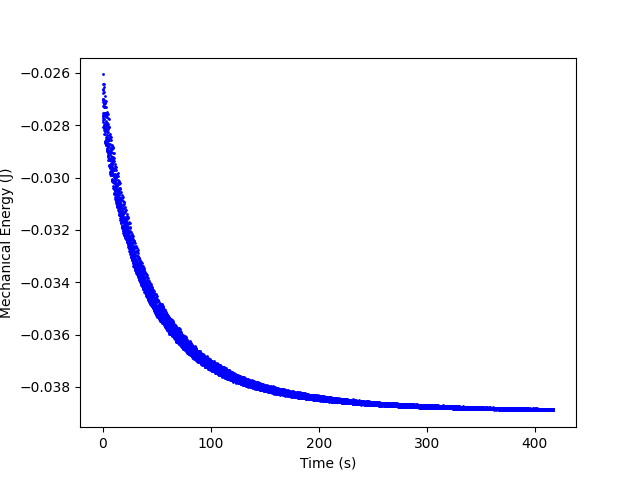
\includegraphics[width=0.5\linewidth]{mechanical-energy}
                    \caption{Mechanical energy over time}
                    \label{fig:mechanical-energy}
                \end{figure}
                
                In this case, mechanical energy is negative because gravitational potential energy is more negative than the sum of spring potential energy and kinetic energy.
                This is because gravitational potential energy only has meaning when compared to other points.
                In other words, the units on the y-axis are only of value when compared to each other, not when compared to 0.
        
        \subsection{Calculating the rate of change of mechanical energy with respect to time}\label{subsec:calculating-the-rate-of-change-of-mechanical-energy-over-time}
            Since potential energy is relevant only when compared to other points, and since the mechanical energy is the sum of potential energy and kinetic energy, the mechanical energy is also only relevant when compared to other points.
            
            %todo do i talk about how it should be stairstep or do i just fit a graph?
            
            If we look between $t=0$ seconds and $t=10$ seconds, we can see that the mechanical energy is decreasing very quickly.
            If we take the average mechanical energy of the first cycle and the average mechanical energy of the last cycle in this range, we can determine the rate of change of mechanical energy over time at around $t = 5$ seconds.
            
            
            The following data is the time, position, velocity, and mechanical energy of the points on the first cycle:
            %table of data
            \begin{table}[H]
                \centering
                \small
                \begin{tabular}{|c|c|c|c|}
                    \hline
                    Time [s] & Position [m] & Velocity [m/s] & Mechanical Energy [J] \\
                    \hline
                    0.00     & 0.291        & -0.006         & -0.026                \\
                    \hline
                    0.05     & 0.281        & -0.289         & -0.027                \\
                    \hline
                    0.10     & 0.257        & -0.467         & -0.028                \\
                    \hline
                    0.15     & 0.227        & -0.478         & -0.028                \\
                    \hline
                    0.20     & 0.202        & -0.319         & -0.027                \\
                    \hline
                    0.25     & 0.191        & -0.046         & -0.027                \\
                    \hline
                    0.30     & 0.197        & 0.243          & -0.027                \\
                    \hline
                    0.35     & 0.218        & 0.447          & -0.028                \\
                    \hline
                    0.40     & 0.248        & 0.490          & -0.028                \\
                    \hline
                    0.45     & 0.275        & 0.354          & -0.027                \\
                    \hline
                    0.50     & 0.289        & 0.094          & -0.026                \\
                    \hline
                \end{tabular}
                \caption{Data for the first cycle}\label{tab:first-cycle-mechanical-energy-table}
            \end{table}
            
            We can then take the average of the mechanical energy for the first cycle as follows using the data from table~\ref{tab:first-cycle-mechanical-energy-table}:
            
            \begin{equation}
                \small
                \begin{aligned}
                    M_{\text{avg, 0}} &= \frac{M_1 + M_2 + M_3 + M_4 + M_5 + M_6 + M_7 + M_8 + M_9 + M_{10} + M_{11}}{11} \\
                    M_{\text{avg, 0}} &= \frac{-0.026 -0.027 -0.028 -0.028 -0.027 -0.027 -0.027 -0.028 -0.028 -0.027 -0.026}{11} \\
                    M_{\text{avg, 0}} &= -0.027 \text{ J} \\
                \end{aligned}\label{eq:average-mechanical-energy-first-cycle}
            \end{equation}
            
            Similarly, we can analyze the last cycle before 10 seconds:
            
            %table of data
            \begin{table}[H]
                \small
                \centering
                \begin{tabular}{|c|c|c|c|}
                    \hline
                    Time [s] & Position [m] & Velocity [m/s] & Mechanical Energy [J] \\
                    \hline
                    9.30     & 0.285        & -0.010         & -0.029                \\
                    \hline
                    9.35     & 0.276        & -0.259         & -0.029                \\
                    \hline
                    9.40     & 0.255        & -0.414         & -0.030                \\
                    \hline
                    9.45     & 0.228        & -0.422         & -0.030                \\
                    \hline
                    9.50     & 0.206        & -0.280         & -0.030                \\
                    \hline
                    9.55     & 0.196        & -0.037         & -0.029                \\
                    \hline
                    9.60     & 0.202        & 0.219          & -0.030                \\
                    \hline
                    9.65     & 0.221        & 0.397          & -0.030                \\
                    \hline
                    9.70     & 0.248        & 0.435          & -0.030                \\
                    \hline
                    9.75     & 0.272        & 0.315          & -0.029                \\
                    \hline
                    9.80     & 0.284        & 0.080          & -0.029                \\
                    \hline
                    9.85     & 0.281        & -0.182         & -0.029                \\
                    \hline
                \end{tabular} %todo does it matter that its slightly more than 1 cycle
                \caption{Data for the last cycle before 10 seconds}\label{tab:last-cycle-before-10-seconds-mechanical-energy-table}
            \end{table}

%            Using the data in table~\ref{tab:last-cycle-before-10-seconds-mechanical-energy-table}, we can calculate the average mechanical energy of the last cycle before 10 seconds as follows:
            
            \begin{equation}
                \small
                \begin{aligned}
                    M_{\text{avg, 9.3}} &= \frac{M_1 + M_2 + M_3 + M_4 + M_5 + M_6 + M_7 + M_8 + M_9 + M_{10} + M_{11} + M_{12}}{12} \\
                    M_{\text{avg, 9.3}} &= \frac{-0.029 -0.029 -0.030 -0.030 -0.030 -0.029 -0.030 -0.030 -0.030 -0.029 -0.029 -0.029}{12} \\
                    M_{\text{avg, 9.3}} &= -0.030 \text{ J} \\
                \end{aligned}\label{eq:average-mechanical-energy-last-cycle-before-10-seconds}
            \end{equation}
            
            Therefore, using the data from equation~\ref{eq:average-mechanical-energy-first-cycle} and equation~\ref{eq:average-mechanical-energy-last-cycle-before-10-seconds}, we can calculate the rate of change of mechanical energy over time at around $t = 5$ seconds as follows:
            
            \begin{equation}
                \small
                \begin{aligned}
                    \frac{\Delta M}{\Delta t} &= \frac{M_{\text{avg, 9.3}} - M_{\text{avg, 0}}}{9.3 \text{ s} - 0 \text{ s}} \\
                    \frac{\Delta M}{\Delta t} &= \frac{-0.030 \text{ J} - (-0.027 \text{ J})}{9.3 \text{ s} - 0 \text{ s}} \\
                    \frac{\Delta M}{\Delta t} &= \frac{-0.003 \text{ J}}{9.3 \text{ s}} \\
                    \frac{\Delta M}{\Delta t} &= -0.000322 \text{ W} \\
                \end{aligned}\label{eq:rate-of-change-of-mechanical-energy-over-time}
            \end{equation}
            
            Therefore, the rate of change of mechanical energy over time at around $t = 5$ seconds is $-0.000322 \text{ W}$. \\
            Using this information, we can graph a line of best fit for the change in mechanical energy over time.
            \newline \indent Since the mechanical energy is $t=5$ seconds is $-0.029 \text{ J}$ (from section~\ref{subsec:calculating-the-mechanical-energy}), and $\frac{\Delta M}{\Delta t}$ from equation~\ref{eq:rate-of-change-of-mechanical-energy-over-time}, we can find the equation of the line of best fit:
            \begin{equation}
                \small
                \begin{aligned}
                    y &= mx + b \\
                    y &= \frac{\Delta M}{\Delta t}x + b \\
                    b &= y - \frac{\Delta M}{\Delta t}x \\
                    b &= -0.029 \text{ J} - (-0.000322 \text{ W})(5 \text{ s}) \\
                    b &= -0.027 \text{ J} \\
                \end{aligned}\label{eq:line-of-best-fit-equation}
            \end{equation}
            Using the value of b from equation~\ref{eq:line-of-best-fit-equation}, we can calculate the equation of the line of best fit as follows:
            \begin{equation}
                \small
                \begin{aligned}
                    y &= mx + b \\
                    y &= \frac{\Delta M}{\Delta t}x + b \\
                    y &= -0.000322 \text{ W}x - 0.027 \text{ J} \\
                \end{aligned}\label{eq:line-of-best-fit-equation-around-5-seconds}
            \end{equation}
            
            This can be visualized on the graph below:
            
            %figure mechanical-energy-linear-fit-5s
            \begin{figure}[H]
                \centering
                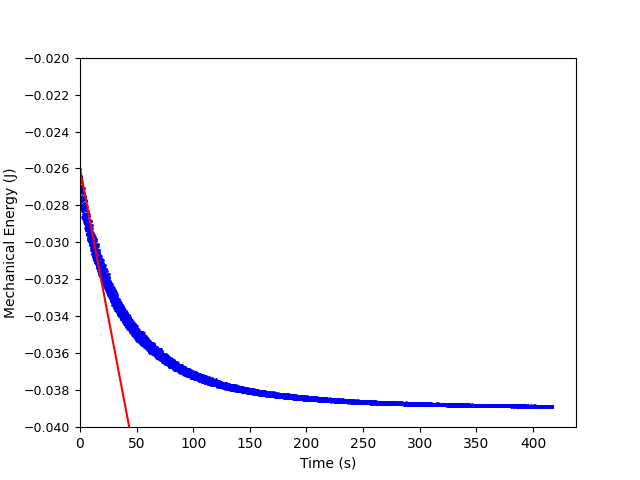
\includegraphics[width=0.5\linewidth]{mechanical-energy-linear-fit-5s}
                \caption{Mechanical energy over time with linear fit around $t=5$ seconds}
                \label{fig:mechanical-energy-linear-fit-5s}
            \end{figure}
            
            In figure~\ref{fig:mechanical-energy-linear-fit-5s} even though the line of best fit is relatively accurate for the first 25 seconds, it rapidly does not become accurate due to the fact that the rate of change of mechanical energy with respect to time is not constant.
            
            To best demonstrate the change in the rate of change of mechanical energy with respect to time we can calculate the linear line of best fit for 2 more positions on the graph, the first one around $t=100$ seconds, and the second one around $t=300$ seconds.\\
            \newline \indent To calculate the linear line of best fit around $t=100$ seconds, we will use the cycle following $t=75$ seconds and the cycle before $t=125$ seconds.
            
            The following table contains the mechanical energy data for the cycle after $t=75$ seconds:
            
            %table of data
            \begin{table}[H]
                \small
                \centering
                \begin{tabular}{|c|c|c|c|}
                    \hline
                    Time [s] & Position [m] & Velocity [m/s] & Mechanical Energy [J] \\
                    \hline
                    75.40    & 0.264        & -0.008         & -0.0361               \\
                    \hline
                    75.45    & 0.259        & -0.139         & -0.0362               \\
                    \hline
                    75.50    & 0.248        & -0.220         & -0.0365               \\
                    \hline
                    75.55    & 0.234        & -0.222         & -0.0366               \\
                    \hline
                    75.60    & 0.222        & -0.144         & -0.0365               \\
                    \hline
                    75.65    & 0.217        & -0.014         & -0.0364               \\
                    \hline
                    75.70    & 0.221        & 0.120          & -0.0365               \\
                    \hline
                    75.75    & 0.231        & 0.211          & -0.0366               \\
                    \hline
                    75.80    & 0.245        & 0.227          & -0.0365               \\
                    \hline
                    75.85    & 0.257        & 0.162          & -0.0363               \\
                    \hline
                    75.90    & 0.264        & 0.038          & -0.0360               \\
                    \hline
                \end{tabular}
                \caption{Data for the cycle at $t=75$ seconds}\label{tab:cycle-at-75-seconds-mechanical-energy-table}
            \end{table}
            
            Using the data from table~\ref{tab:cycle-at-75-seconds-mechanical-energy-table}, we can calculate the average mechanical energy of the cycle at $t=75$ seconds:
            
            \begin{equation}
                \small
                \begin{aligned}
                    M_{\text{avg, 75}} &= \frac{M_1 + M_2 + M_3 + M_4 + M_5 + M_6 + M_7 + M_8 + M_9 + M_{10} + M_{11}}{11} \\
                    M_{\text{avg, 75}} &= \frac{-0.0361 -0.0362 -0.0363 -0.0364 -0.0365 \times 4 -0.0366 \times 2 -0.0360}{11} \\ %todo is this formatting ok
                    M_{\text{avg, 75}} &= -0.0364 \text{ J} \\
                \end{aligned}\label{eq:average-mechanical-energy-cycle-at-75-seconds}
            \end{equation}
            
            The following table contains the mechanical energy data for the cycle before $t=125$ seconds:
            
            %table of data
            \begin{table}[H]
                \small
                \centering
                \begin{tabular}{|c|c|c|c|}
                    \hline
                    Time [s] & Position [m] & Velocity [m/s] & Mechanical Energy [J] \\
                    \hline
                    124.45   & 0.256        & -0.032         & -0.0375               \\
                    \hline
                    124.50   & 0.251        & -0.116         & -0.0377               \\
                    \hline
                    124.55   & 0.243        & -0.158         & -0.0378               \\
                    \hline
                    124.60   & 0.233        & -0.144         & -0.0378               \\
                    \hline
                    124.65   & 0.226        & -0.078         & -0.0378               \\
                    \hline
                    124.70   & 0.224        & 0.016          & -0.0377               \\
                    \hline
                    124.75   & 0.228        & 0.104          & -0.0378               \\
                    \hline
                    124.80   & 0.236        & 0.156          & -0.0378               \\
                    \hline
                    124.85   & 0.246        & 0.151          & -0.0377               \\
                    \hline
                    124.90   & 0.254        & 0.090          & -0.0376               \\
                    \hline
                    124.95   & 0.256        & -0.002         & -0.0376               \\
                    \hline
                \end{tabular}
                \caption{Data for the cycle at $t=125$ seconds}\label{tab:cycle-at-125-seconds-mechanical-energy-table}
            \end{table}
            Using the data from table~\ref{tab:cycle-at-125-seconds-mechanical-energy-table}, we can calculate the average mechanical energy of the cycle at $t=125$ seconds as follows:
            
            \begin{equation}
                \small
                \begin{aligned}
                    M_{\text{avg, 125}} &= \frac{M_1 + M_2 + M_3 + M_4 + M_5 + M_6 + M_7 + M_8 + M_9 + M_{10} + M_{11}}{11} \\
                    M_{\text{avg, 125}} &= \frac{-0.0375 -0.0376 \times 2 -0.0377 \times 3 -0.0378 \times 5 }{11} \\
                    M_{\text{avg, 125}} &= -0.0377 \text{ J} \\
                \end{aligned}\label{eq:average-mechanical-energy-cycle-at-125-seconds}
            \end{equation}
            
            At $t=100$ seconds from section~\ref{subsec:calculating-the-mechanical-energy}, the mechanical energy is $-0.0373 \text{ J}$.
            With the average mechanical energy for the cycle before $t=125$ seconds and the cycle after $t=75$ seconds, we can calculate the rate of change of mechanical energy over time at around $t=100$ seconds as follows:
            
            \begin{equation}
                \small
                \begin{aligned}
                    \frac{\Delta M}{\Delta t} &= \frac{M_{\text{avg, 125}} - M_{\text{avg, 75}}} {125 \text{ s} - 75 \text{ s}} \\
                    \frac{\Delta M}{\Delta t} &= \frac{-0.0377 \text{ J} - (-0.0364 \text{ J})} {125 \text{ s} - 75 \text{ s}} \\
                    \frac{\Delta M}{\Delta t} &= \frac{-0.0013 \text{ J}} {50 \text{ s}} \\
                    \frac{\Delta M}{\Delta t} &= -0.000026 \text{ W} \\
                \end{aligned}\label{eq:rate-of-change-of-mechanical-energy-over-time-around-100-seconds}
            \end{equation}
            
            
            Therefore, the rate of change of mechanical energy over time at around $t=100$ seconds is $-0.000026 \text{ W}$.
            Using this information, we can calculate the equation of the line of best fit around $t=100$ seconds:
            
            \begin{equation}
                \small
                \begin{aligned}
                    y &= mx + b \\
                    y &= \frac{\Delta M}{\Delta t}x + b \\
                    y &= -0.000026 \text{ W}x + b \\
                    b &= y - (-0.000026 \text{ W}x)\\
                    b &= -0.0373 \text{ J} - (-0.000026 \text{ W})(100 \text{ s}) \\
                    b &= -0.0347 \text{ J} \\
                \end{aligned}\label{eq:line-of-best-fit-b-around-100-seconds}
            \end{equation}
            
            Using equations~\ref{eq:rate-of-change-of-mechanical-energy-over-time-around-100-seconds} and~\ref{eq:line-of-best-fit-b-around-100-seconds}, the line of best fit around $t=100$ seconds has the equation:
            
            \begin{equation}
                \small
                \begin{aligned}
                    y &= mx + b \\
                    y &= \frac{\Delta M}{\Delta t}x + b \\
                    y &= -0.000026 \text{ W}x - 0.0347 \text{ J} \\
                \end{aligned}\label{eq:line-of-best-fit-equation-around-100-seconds}
            \end{equation}
            
            If we graph that line of best fit on the graph of mechanical energy, we get the following graph:
            
            %figure mechanical-energy-linear-fit-100s
            \begin{figure}[H]
                \centering
                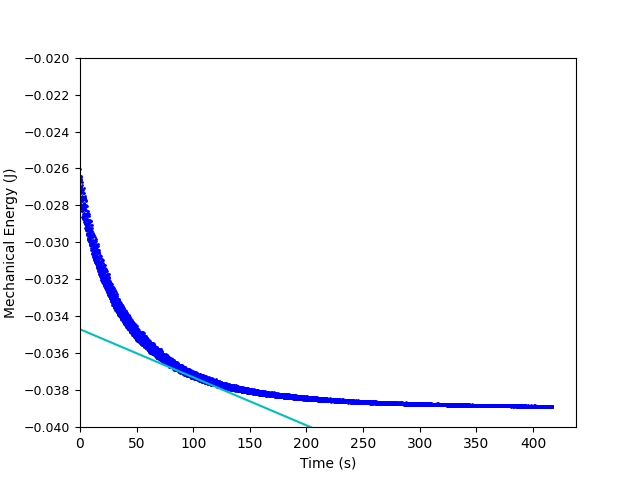
\includegraphics[width=0.49\linewidth]{mechanical-energy-linear-fit-100s}
                \caption{Mechanical energy over time with linear fit around $t=100$ seconds}
                \label{fig:mechanical-energy-linear-fit-100s}
            \end{figure}
            
            Even though this linear line of best fit is relatively accurate around $t=100$ seconds, it is not accurate for the rest of the graph, due to the fact that the rate of change of mechanical energy over time is not constant.
            In fact, as soon as the time is greater than $t=125$ seconds or less than $t=75$ seconds, the line of best fit is already significantly inaccurate.
            This is very similar to the previous line of best fit, but the slope of this line of best fit is less steep (closer to 0), meaning the rate of change of mechanical energy over time is changing, becoming less negative.
            
            The last line of best fit that we will calculate is the one around $t=300$ seconds. To calculate this line of best fit, we will use the cycle after $t=250$ seconds, the cycle that includes $t=300$ seconds, and the cycle before $t=350$ seconds.
            
            The following table contains the mechanical energy data for the cycle after $t=250$ seconds:
            
            %table of data
            \begin{table}[H]
                \small
                \centering
                \begin{tabular}{|c|c|c|c|}
                    \hline
                    Time [s] & Position [m] & Velocity [m/s] & Mechanical Energy [J] \\
                    \hline
                    250.35   & 0.248        & 0.002          & -0.03858              \\
                    \hline
                    250.40   & 0.247        & -0.045         & -0.03860              \\
                    \hline
                    250.45   & 0.243        & -0.075         & -0.03864              \\
                    \hline
                    250.50   & 0.238        & -0.076         & -0.03867              \\
                    \hline
                    250.55   & 0.234        & -0.051         & -0.03868              \\
                    \hline
                    250.60   & 0.232        & -0.008         & -0.03868              \\
                    \hline
                    250.65   & 0.233        & 0.041          & -0.03866              \\
                    \hline
                    250.70   & 0.237        & 0.073          & -0.03868              \\
                    \hline
                    250.75   & 0.242        & 0.077          & -0.03866              \\
                    \hline
                    250.80   & 0.246        & 0.055          & -0.03862              \\
                    \hline
                    250.85   & 0.248        & 0.013          & -0.03859              \\
                    \hline
                \end{tabular}
                \caption{Data for the cycle at $t=250$ seconds}\label{tab:cycle-at-250-seconds-mechanical-energy-table}
            \end{table}
            
            From table~\ref{tab:cycle-at-250-seconds-mechanical-energy-table}, we can calculate the average mechanical energy of the cycle at $t=250$ seconds:
            
            \begin{equation}
                \small
                \begin{aligned}
                    M_{\text{avg, 250}} &= \frac{M_1 + M_2 + M_3 + M_4 + M_5 + M_6 + M_7 + M_8 + M_9 + M_{10} + M_{11}}{11} \\
                    M_{\text{avg, 250}} &= \frac{-0.03858 -0.03859 -0.03860 -0.03862 -0.03864 -0.03866 \times 2 -0.03867 -0.03868 \times 3 }{11} \\
                    M_{\text{avg, 250}} &= -0.03865 \text{ J} \\
                \end{aligned}\label{eq:average-mechanical-energy-cycle-at-250-seconds}
            \end{equation}
            
            The following table contains the mechanical energy data for the cycle before $t=350$ seconds:
            
            %table of data
            \begin{table}[H]
                \small
                \centering
                \begin{tabular}{|c|c|c|c|}
                    \hline
                    Time [s] & Position [m] & Velocity [m/s] & Mechanical Energy [J] \\
                    \hline
                    349.40   & 0.245        & 0.007          & -0.03879              \\
                    \hline
                    349.45   & 0.245        & -0.024         & -0.03879              \\
                    \hline
                    349.50   & 0.243        & -0.045         & -0.03882              \\
                    \hline
                    349.55   & 0.240        & -0.050         & -0.03884              \\
                    \hline
                    349.60   & 0.237        & -0.037         & -0.03884              \\
                    \hline
                    349.65   & 0.235        & -0.011         & -0.03885              \\
                    \hline
                    349.70   & 0.236        & 0.018          & -0.03885              \\
                    \hline
                    349.75   & 0.238        & 0.040          & -0.03885              \\
                    \hline
                    349.80   & 0.240        & 0.049          & -0.03884              \\
                    \hline
                    349.85   & 0.243        & 0.040          & -0.03882              \\
                    \hline
                    349.90   & 0.245        & 0.017          & -0.03880              \\
                    \hline
                    349.95   & 0.245        & -0.011         & -0.03880              \\
                    \hline
                \end{tabular}
                \caption{Data for the cycle at $t=350$ seconds}\label{tab:cycle-at-350-seconds-mechanical-energy-table}
            \end{table}
            
            From table~\ref{tab:cycle-at-350-seconds-mechanical-energy-table}, we can calculate the average mechanical energy of the cycle at $t=350$ seconds:
            
            \begin{equation}
                \small
                \begin{aligned}
                    M_{\text{avg, 350}} &= \frac{M_1 + M_2 + M_3 + M_4 + M_5 + M_6 + M_7 + M_8 + M_9 + M_{10} + M_{11} + M_{12}}{12} \\
                    M_{\text{avg, 350}} &= \frac{-0.03879 -0.03880 \times 2 -0.03882 \times 2 -0.03884 \times 3 -0.03885 \times 4}{12} \\
                    M_{\text{avg, 350}} &= -0.03883 \text{ J} \\
                \end{aligned}\label{eq:average-mechanical-energy-cycle-at-350-seconds}
            \end{equation}
            
            Now that we have the average mechanical energy for the cycle before $t=350$ seconds and the cycle after $t=250$ seconds, we can calculate the rate of change of mechanical energy over time at around $t=300$ seconds as follows:
            
            \begin{equation}
                \small
                \begin{aligned}
                    \frac{\Delta M}{\Delta t} &= \frac{M_{\text{avg, 350}} - M_{\text{avg, 250}}} {350 \text{ s} - 250 \text{ s}} \\
                    \frac{\Delta M}{\Delta t} &= \frac{-0.03883 \text{ J} - (-0.03865 \text{ J})} {350 \text{ s} - 250 \text{ s}} \\
                    \frac{\Delta M}{\Delta t} &= \frac{-0.00018 \text{ J}} {100 \text{ s}} \\
                    \frac{\Delta M}{\Delta t} &= -0.0000018 \text{ W} \\
                \end{aligned}\label{eq:rate-of-change-of-mechanical-energy-over-time-around-300-seconds}
            \end{equation}
            
            Therefore, the rate of change of mechanical energy over time at around $t=300$ seconds is $-0.0000018 \text{ W}$.
            At $t=300$ seconds, from section~\ref{subsec:calculating-the-mechanical-energy}, the mechanical energy is $-0.03877 \text{ J}$.
            Using this information, we can calculate the equation of the line of best fit around $t=300$ seconds as follows:
            
            \begin{equation}
                \small
                \begin{aligned}
                    y &= mx + b \\
                    y &= \frac{\Delta M}{\Delta t}x + b \\
                    y &= -0.0000018 \text{ W}x + b \\
                    b &= y - (-0.0000018 \text{ W}x) \\
                    b &= -0.03877 \text{ J} - (-0.0000018 \text{ W})(300 \text{ s}) \\
                    b &= -0.03823 \text{ J} \\
                \end{aligned}\label{eq:line-of-best-fit-b-around-300-seconds}
            \end{equation}
            
            Using equations~\ref{eq:rate-of-change-of-mechanical-energy-over-time-around-300-seconds} and~\ref{eq:line-of-best-fit-b-around-300-seconds}, we can calculate the equation of the line of best fit around $t=300$ seconds:
            \begin{equation}
                \small
                \begin{aligned}
                    y &= mx + b \\
                    y &= \frac{\Delta M}{\Delta t}x + b \\
                    y &= -0.0000018 \text{ W}x - 0.03823 \text{ J} \\
                \end{aligned}\label{eq:line-of-best-fit-equation-around-300-seconds}
            \end{equation}
            
            If we graph that line of best fit on the graph of mechanical energy, we get the following graph:
            
            %figure mechanical-energy-linear-fit-300s
            \begin{figure}[H]
                \centering
                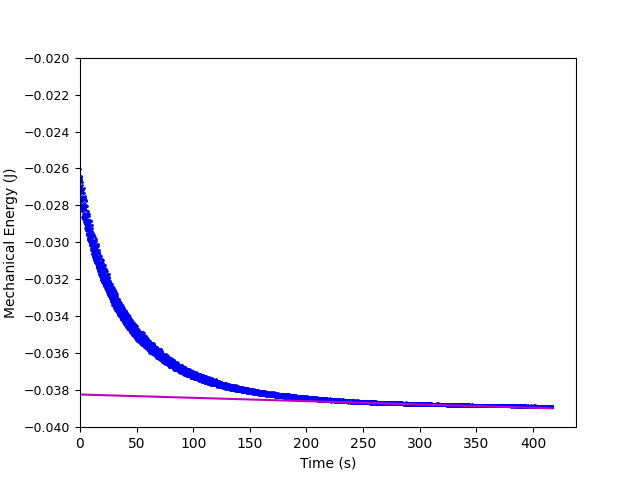
\includegraphics[width=0.47\linewidth]{mechanical-energy-linear-fit-300s}
                \caption{Mechanical energy over time with linear fit around $t=300$ seconds}
                \label{fig:mechanical-energy-linear-fit-300s}
            \end{figure}
            
            Even though this linear line of best fit is relatively accurate around $t=300$ seconds, it is not accurate for the rest of the graph, due to the fact that the rate of change of mechanical energy over time is not constant.
            However, unlike the previous graphs, this line of best fit is accurate for a longer period of time, since the rate of change of mechanical energy over time is more constant around $t=300$ seconds than it is around $t=100$ seconds.
            This line of best fit is accurate from approximately 200 seconds all the way to 400 seconds.
            This is because as the mechanical energy falls, the maximum velocity of the mass decreases, which means there is less energy loss, causing the mechanical energy to start to resemble a linear trend after 200 seconds.
            
            The differences in the rate of change of mechanical energy with respect to time is even more evident when we compare the rate of change of mechanical energy over time for all three of the linear fits that we calculated:
            
            %figure mechanical-energy-linear-fit-all
            \begin{figure}[H]
                \centering
                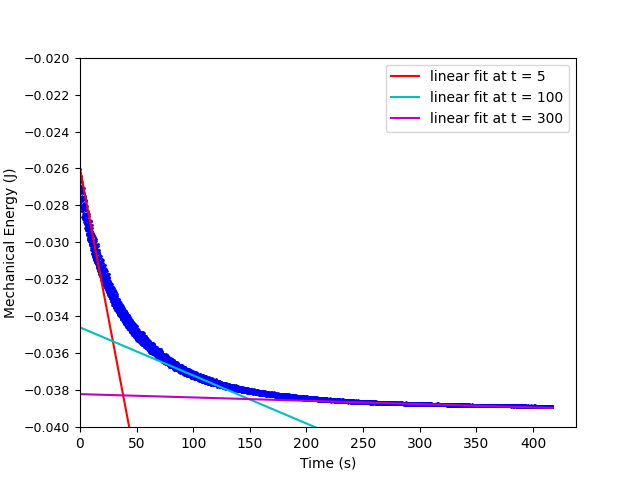
\includegraphics[width=0.46\linewidth]{mechanical-energy-linear-fit-all}
                \caption{Mechanical energy over time with linear fit around $t=100$ seconds}
                \label{fig:mechanical-energy-linear-fit-all}
            \end{figure}
            
            In this figure it is obvious that the rate of change of mechanical energy over time is not constant, and that it is decreasing over time.
            The linear fit at $t=5$ seconds is significantly steeper than the linear fit at $t=300$ seconds.
            This shows that the rate of change of the mechanical energy of the oscillating mass with respect to time is always decreasing.
            This is because as the mechanical energy falls, the maximum velocity of the mass decreases, which means there is less energy loss due to air resistence, as energy lost due to air resistance is proportional to the velocity.
            
            The prior process can be repeated for every point on the graph of mechanical energy over time, and a line of best fit can be calculated for each point.
            The following graph, for each point takes the mechanical energy of the point 2.8 seconds before and 2.8 seconds after, and graphs the rate of change of mechanical energy over time for that point.
            
            \begin{minipage}{.5\textwidth}
                %figure mechanical-energy-rate-of-change
                \begin{figure}[H]
                    \centering
                    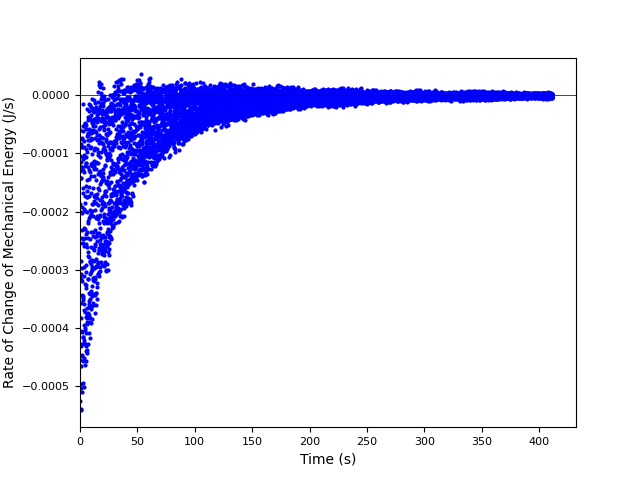
\includegraphics[width=0.92\linewidth]{mechanical-energy-rate-of-change}
                    \small \caption{ \small Rate of change of mechanical energy over time}
                    \label{fig:mechanical-energy-rate-of-change}
                \end{figure}
            \end{minipage}%
            \begin{minipage}{.5\textwidth}
                %figure velocity
                \begin{figure}[H]
                    \centering
                    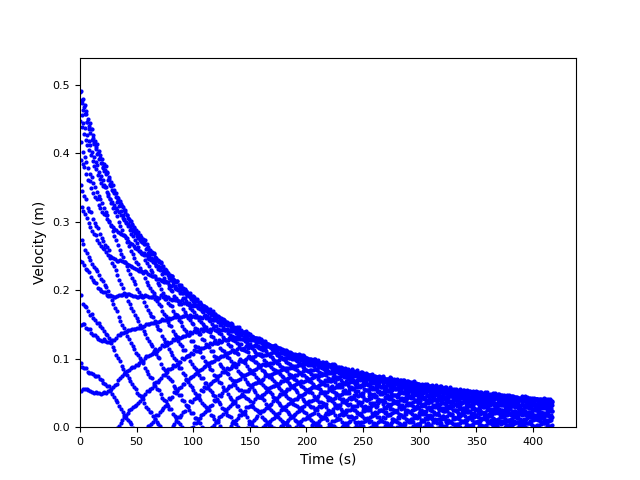
\includegraphics[width=0.92\linewidth]{velocity}
                    \small \caption{ \small Velocity over time}
                    \label{fig:velocity1}
                \end{figure}
            \end{minipage}
            
            The mechanical energy over time graph shows that the mechanical energy is always decreasing, and that the rate of change of mechanical energy over time is not constant.
            The magnitude of the change in mechanical energy near the end of the graph is significantly less than the maximum magnitude of the change in mechanical energy near the beginning of the graph, most likely due to the fact that the velocity of the mass is decreasing, and thus the energy loss to air resistance is decreasing.
            
            When comparing the velocity from figure~\ref{fig:velocity1} to the rate of change of mechanical energy over time from figure~\ref{fig:mechanical-energy-rate-of-change}, it is evident that the rate of change of mechanical energy over time is proportional to the velocity.
            At time $t=0$ seconds, the velocity is at its maximum, and the mechanical energy is decreasing the fastest, at $t=50$ seconds, the velocity has decreased a significant amount, and the magnitude of the rate at which mechanical energy is decreasing is less than at $t=0$ seconds.
            When $t=100$ seconds, the velocity is even lower than at $t=50$ seconds, and the magnitude of the rate of change of mechanical energy over time is even less than at $t=50$ seconds.
            At $t=300$ seconds, the velocity is at nearly its lowest, and the magnitude of the rate of change of mechanical energy over time is at nearly its lowest.
            This demonstrates a strong correlation between the two variables, as velocity decreases, the magnitude of the rate of change of mechanical energy over time decreases.
    
    
    \section{Discussion}\label{sec:discussion}
%    \subsection{Calculating the Average Rate of Change of Mechanical Energy Over Time}
        
        \subsection{Question 1:}\label{subsec:question-1}
            
            \subsubsection{Question 1a: Give the experimental average value for the rate of change of the mechanical energy of the oscillating mass with respect to time?}
                If we take the average of all the rates of change of mechanical energy over time from figure~\ref{fig:mechanical-energy-rate-of-change}, we get that the average rate of change of mechanical energy is $-0.000026 \text{ W}$.
                %todo that number seems wrong
                This means that over the course of the experiment, the rate of change of mechanical energy was on average $-0.000026 \text{ W}$.
                
                At $t=0$ seconds the mechanical energy is $-0.02605 \text{ J}$, and at $t=417.15$ seconds the mechanical energy is $-0.03886 \text{ J}$.
                The slope between these two points is solved as follows:
                
                \begin{equation}
                    \small
                    \begin{aligned}
                        \frac{\Delta M}{\Delta t} &= \frac{M_2 - M_1}{t_2 - t_1} \\
                        \frac{\Delta M}{\Delta t} &= \frac{-0.03886 \text{ J} - (-0.02605 \text{ J})}{417.15 \text{ s} - 0 \text{ s}} \\
                        \frac{\Delta M}{\Delta t} &= \frac{-0.01281 \text{ J}}{417.15 \text{ s}} \\
                        \frac{\Delta M}{\Delta t} &= -0.000027 \text{ W} \\
                    \end{aligned}\label{eq:rate-of-change-of-mechanical-energy-over-time-overall}
                \end{equation}
                
                %figure average-spring-energy
                \begin{figure}[H]
                    \centering
                    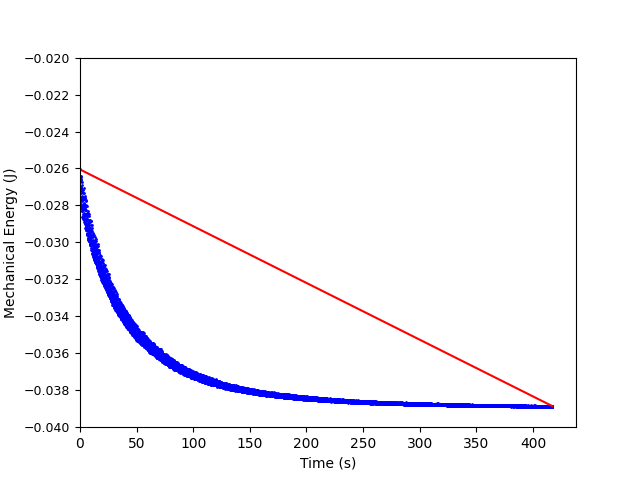
\includegraphics[width=0.5\linewidth]{average-spring-energy}
                    \caption{Average rate of change of the mechanical energy of the oscillating mass with respect to time}
                    \label{fig:average-spring-energy}
                \end{figure}
                
                These two values are close enough to be considered effectively the same.
                Thus the experimental average value for the rate of change of the mechanical energy of the oscillating mass with respect to time over the course of the 417.15 seconds the mass oscillated for is $-0.000027 \text{ W}$.
            
            \subsubsection{Question 1b: What is your experimental rate of change of the mechanical energy of the oscillating mass with respect to time?}
                The rate of change of mechanical energy of the mass with respect to time depends based on the time.
                Based on figure~\ref{fig:mechanical-energy-rate-of-change} (reproduced below), the rate of change of mechanical energy of the experimental rate of change of the mechanical energy of the oscillating mass with respect to time changes.
                
                %figure mechanical-energy-rate-of-change
                \begin{figure}[H]
                    \centering
                    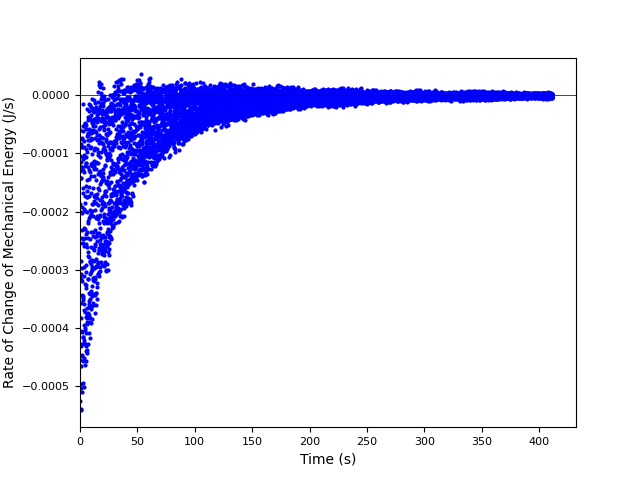
\includegraphics[width=0.5\linewidth]{mechanical-energy-rate-of-change}
                    \caption{Mechanical energy over time, using a radius of 2.8 seconds}
                    \label{fig:mechanical-energy-rate-of-change-2}
                \end{figure}
                
                The graph shows that the mechanical energy is always decreasing, and that the rate of change of mechanical energy with respect to time is not constant.
                The magnitude of the change in mechanical energy near the end of the graph is significantly less than the maximum magnitude of the change in mechanical energy near the beginning of the graph, most likely due to the fact that the velocity of the mass is decreasing, and thus the energy loss to air resistance is decreasing.
                
                At time $t=0$ seconds, the mechanical energy is decreasing the fastest, while at $t=50$ seconds, the magnitude of the rate at which mechanical energy is decreasing is less than at $t=0$ seconds.
                When $t=100$ seconds, the magnitude of the rate of change of mechanical energy over time is even less than at $t=50$ seconds.
                At $t=300$ seconds, the magnitude of the rate of change of mechanical energy over time is at nearly its lowest.
                In other words, as time goes on, the experimental rate of change of mechanical energy of the oscillating mass with respect to time decreases. \\
                
                In addition, an exponential curve fit can be used to find the experimental rate of change of mechanical energy of the oscillating mass with respect to time.
                An exponential curve fit is used because the rate of change of mechanical energy of the oscillating mass with respect to time is decreasing nearly exponentially.
                The following graph shows the exponential curve fit for the rate of change of mechanical energy of the oscillating mass with respect to time:
                
                %figure mechanical-energy-exponential-fit
                \begin{figure}[H]
                    \centering
                    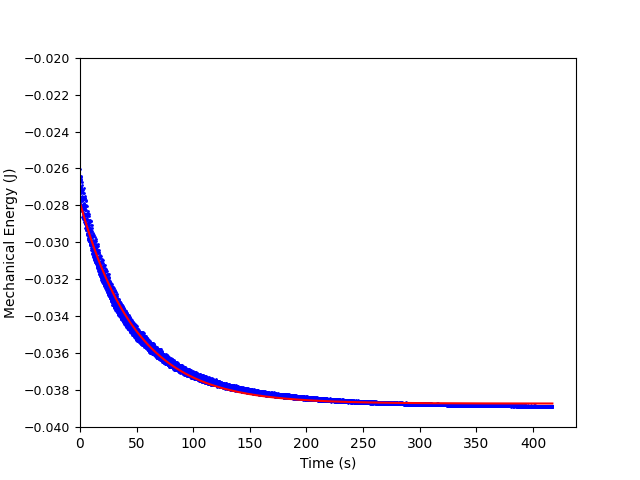
\includegraphics[width=0.5\linewidth]{mechanical-energy-exponential-fit}
                    \caption{Mechanical energy exponential fit}
                    \label{fig:mechanical-energy-exponential-fit}
                \end{figure}

%                M(t) = 0.01086 * 10^(-0.008873 t) - 0.03872
                The function used in the exponential fit is $M(t) = 0.01086 \times 10^{-0.008873 \times t} - 0.03872 \text{ J}$, where $M(t)$ is the mechanical energy of the oscillating mass at time $t$.
                This equation fits the data relatively well, however it smooths out the oscillations in the data, and thus is not a perfect fit.
                At certain points in time, such as when the mass is at the peak, its velocity is 0, and there should be little to no air-resistance, while at other points in time, such as when the mass is at its middle point, its velocity is at its maximum, and there would be a lot of air-resistance.
                The exponential fit averages these changes out to form a line.
                
                
                The derivative of the exponential fit is the rate of change of the mechanical energy of the oscillating mass with respect to time and can be graphed as well.
                
                %figure change-in-mechanical-energy
                \begin{figure}[H]
                    \centering
                    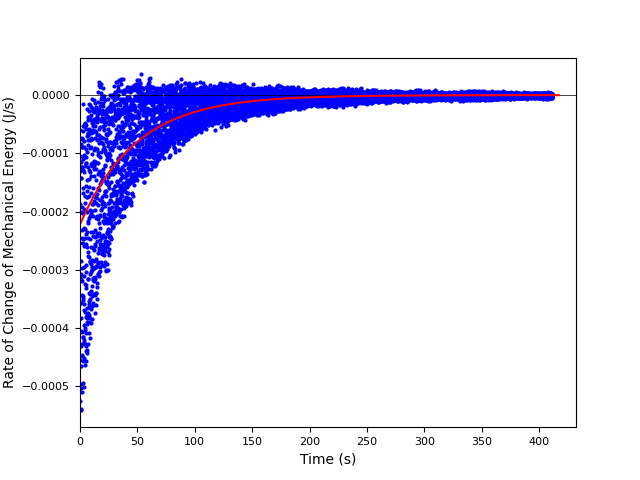
\includegraphics[width=0.5\linewidth]{change-in-mechanical-energy}
                    \caption{Change in mechanical energy over time}
                    \label{fig:change-in-mechanical-energy}
                \end{figure}
                
                The graph shows how the change in mechanical energy with respect to time line is approximately an average of the maximum and minimum points on the rate of change of mechanical energy with respect to time graph.
                By taking the derivative, it is possible to come up with an approximate function for the rate of change of mechanical energy of the oscillating mass with respect to time.
                
                
                
                \begin{equation}
                    \small
                    \begin{aligned}
                        M(t) &= 0.01086 \times 10^{-0.008873 \times t} - 0.03872 \text{ J}\\
                        \frac{d}{dt} M(t) &= \frac{d}{dt} (0.01086 \times 10^{-0.008873 \times t} - 0.03872) \text{ W}\\
                        \frac{dM}{dt} &= 0.01086 \times 10^{-0.008873 \times t} \times \ln(10) \times -0.008873 \text{ W}\\
                        \frac{dM}{dt} &= -0.000222 \times 10^{-0.008873 \times t} \text{ W}\\
                    \end{aligned}\label{eq:rate-of-change-of-mechanical-energy-over-time-exponential-fit}
                \end{equation}
                
                This means that the rate of change of the mechanical energy of the oscillating mass with respect to time $\frac{dM}{dt}$ is approximately $-0.000222 \times 10^{-0.008873 \times t} \text{ W}$.
        
        \subsection{Question 2: What are the energy transformations that are responsible for the change in mechanical energy?}\label{subsec:question-2:-what-are-the-energy-transformations-that-are-responsible-for-the-change-in-mechanical-energy?}
            The change in mechanical energy is caused primarily by air resistance, due to the mass moving through the air.
            There are also some additional minor losses such as friction between the mass holder and the spring.
            The friction in both of these cases converts the mechanical energy of the mass into heat/thermal energy and into the kinetic energy of the air.
            Specifically, it transfers the kinetic energy into heat/thermal energy, causing a decrease in the mechanical energy of the oscillating mass.
            
            Using $W_{\text{ext}} + W_{\text{int,nc}} = \Delta M$, we can see that the change in mechanical energy is caused by the external forces acting upon the system.
            
            The external and internal non-conservative forces are primarily air resistance and friction.
            From the analysis in previous sections, it seems apparent that when velocity is high, the rate of change of mechanical energy is high, and when velocity is low, the rate of change of mechanical energy is low.
            This implies the primary cause of the change in mechanical energy is air resistance, as air resistance is proportional to the velocity of the mass.
            
            In air resistence, the energy transformations that are taking place are the conversion of the mechanical energy of the mass into heat/thermal energy and the kinetic energy of the air.
            Since the thermal energy of the air is the average kinetic energy of the particles in the air, the energy transfer when the object pushes through the air can be expressed as $K_{mass} \longrightarrow K_{air} + E_{th, air}$.
            Furthermore, the small amount of energy transformations that are occurring due to internal friction can be expressed as $K \longrightarrow E_{th}$.
    These energy transformations are the primary cause of the change in mechanical energy.
    
    \section{Strengths, Potential Errors, and Possible Improvements}\label{sec:potential-errors-next-steps-and-future-improvements}
        
        \subsection{Strengths}
            \begin{itemize}
                \item The large amount of data collected allows for more analysis to occur over time.
                \item The data was collected at a high frequency, allowing for more accurate results.
                \item The data was collected using an ultrasonic motion detector, which can detect the position of the mass in all stages of its oscillation.
                \item The ultrasonic motion detector also detected the velocity of the mass, which allowed for more accurate calculations of the mechanical energy.
            \end{itemize}
        
        \subsection{Potential Errors}
            \begin{itemize}
                \item Ultrasonic sensor's readings occur every 0.05 seconds. This means that the velocity readings are not accurate enough, and the acceleration readings are not accurate enough, as when the mass reaches the peak, the sensor may miss it. The sensor tends to give a reading right before the peak and right after.
                \item The mass of the mass holder was not measured.
                \item The spring is not massless.
                \item The spring did not oscillate directly up and down.
                \item The x0 position was not accurate.
                \item Not enough data points were taken to find the spring constant.
                \item Multiple trials were not taken to find the change in mechanical energy over time.
                \item In the change in mechanical energy over time graph, there are points that show that the mechanical energy is sometimes increasing.
                However, there are no external or non-conservative forces that would cause the mechanical energy to increase.
                This is most likely due to the fact that the ultrasonic motion detector's velocity readings were unreliable, and the measurements of x0 and the mass were most likely unreliable as well.
                Having more runs and more reliable readings would help to fix this issue.
            \end{itemize}
        
        \subsection{Possible Improvements}\label{subsec:possible-improvements}
            \begin{itemize}
                \item Running the experiment for a longer period of time would allow for more data to be collected, and would allow for more accurate results.
                \item Running the experiment multiple times would allow for more accurate results.
                \item Using a more accurate ultrasonic motion detector would allow for more accurate results, as with more frequent readings, the velocity and acceleration of the mass would be more accurate.
                In addition, a more accurate ultrasonic motion detector would allow for more accurate readings of the position of the mass, leading to more accurate calculations of the mechanical energy.
                \item Measuring the mass of the mass holder would allow for more accurate calculations of the mechanical energy.
                \item Calculating the effects of the spring's mass would allow for more accurate calculations of the mechanical energy.
                \item Ensuring that the spring that oscillates directly up and down would allow for more accurate calculations of the changes to mechanical energy.
                \item Measuring the surface area of the mass holder would allow for calculations of the air resistance.
                \item Measuring the air density would allow for calculations of the air resistance.
                \item Measuring more datapoints to determine the spring constant would allow for more accurate calculations of the mechanical energy.
                \item Measuring the natural equilibrium point with a ruler would be more accurate and help with increasing accuracy.
            \end{itemize}
    
    
    \section{Conclusion}\label{sec:conclusion}
        In conclusion, the mechanical energy of the oscillating mass decreases over time, and the rate of change of mechanical energy over time is not constant.
        The mechanical energy of the oscillating mass decreases over time due to air resistance, which converts the kinetic energy of the mass into heat/thermal energy as well as kinetic energy.
        The rate of change of mechanical energy over time is not constant because as the mechanical energy falls, the maximum velocity of the mass decreases, which means there is less energy loss.
        From this experiment we can conclude that the mechanical energy of an oscillating mass decreases over time, and that the rate of change of mechanical energy over time is not constant, and is primarily caused by air resistance, due to its correlation with the velocity of the object.
   
\end{document}
